\section{Governing equations}
\label{sec:governing}
The shallow water equations are depth-integrated incompressible Navier-Stokes equations and are given in conservative form by,
\begin{eqnarray}
\label{eq:swe}
\pa{\eta}{t} + \pa{(hu)}{x} + \pa{(hv)}{y} &=& 0, \nonumber \\
\pa{}{t}(hu) + \pa{}{x}\left(hu^2 + \frac{1}{2}gh^2 \right) + \pa{}{y} (huv)&=& - gh\pa{B}{x} - \tau_{bx}, \nonumber \\
\pa{}{t}(hv) + \pa{}{x}(huv) + \pa{}{y}\left( hv^2 + \frac{1}{2}gh^2\right) &=&  -gh\pa{B}{y} - \tau_{by},
\end{eqnarray}
where, $\eta$ is free surface height above mean sea level, $h$ is the fluid column height, $u$, and $v$ are velocity components in longitudinal and latitudinal directions. $B$ is ocean bed topography or bathymetry, and $g$ is the acceleration due to gravity (see Fig. (\ref{fig:notation})  for the notation). $\tau_{bx}$ and $\tau_{by}$ are components of bottom friction force.
\begin{figure}[h!]
  \begin{center}
    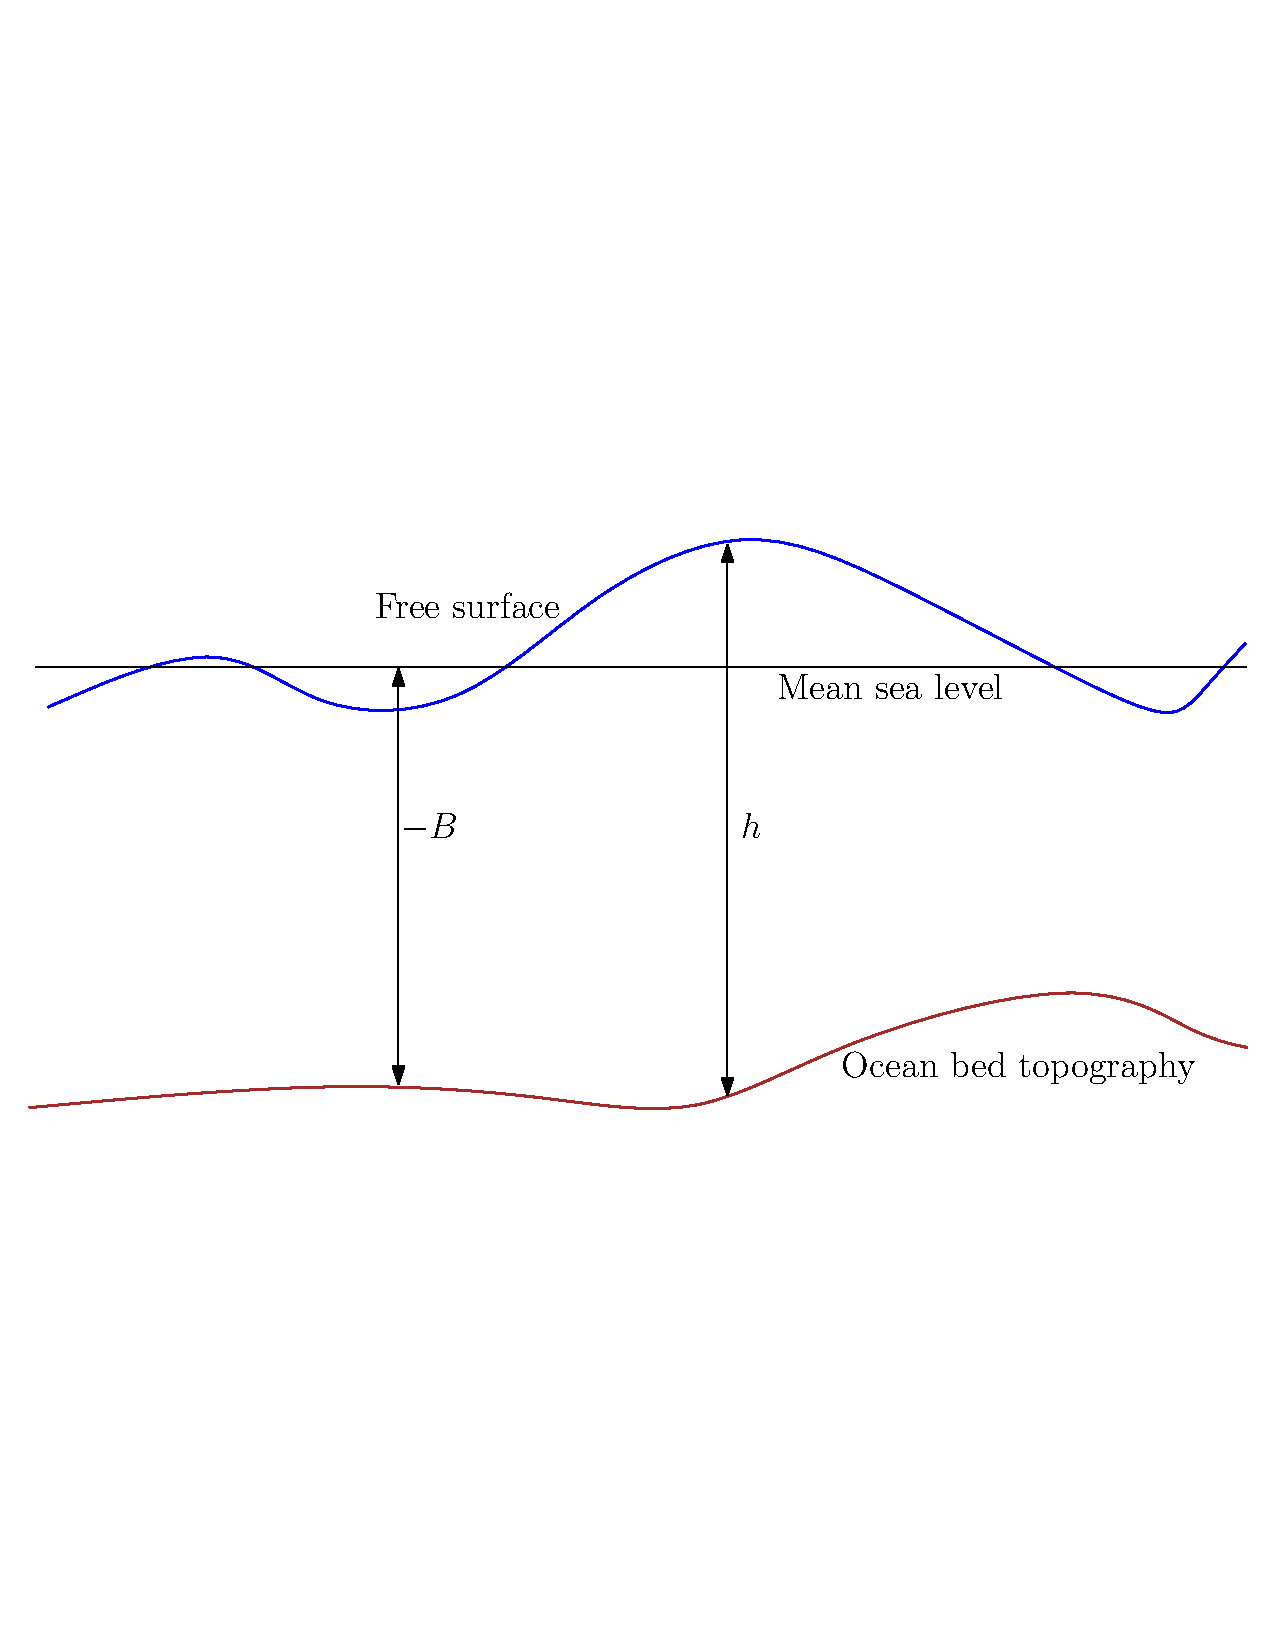
\includegraphics[trim=0cm 8cm 0cm 8cm,clip=true,width=0.5\linewidth]{./figures/bathymetry.pdf}
\caption{Diagram representation of notation of ocean domain.}
\label{fig:notation}
\end{center}
\end{figure}

\noindent In simplified form, these equations are represented as,
\begin{equation}
\label{eq:swe_conservative}
\pa{Q}{t} + \pa{F}{x} + \pa{G}{y} = S,
\end{equation}
here, $Q$ is the state vector, $F$, $G$ are the nonlinear flux vectors, and $S$ is the forcing vector. A high order discontinuous Galerkin method to obtain the solution of  Eq. (\ref{eq:swe_conservative}) and the details are discussed in the following  section.

\section{Numerical scheme}
\label{sec:discretization}
The computational domain   $\Omega \subset \mathbb{R}^2$, is partitioned into a set of non-overlapping, conforming triangles $\{ \Omega = \displaystyle\cup_{k} D^{k} \}$. The solution for $Q$ is approximated by $Q_H$, the components of which belong to the space of discontinuous piecewise polynomial of a given degree $N$ in each element ($P^{N}(D^{k})$). The PDEs in the Eq. (\ref{eq:swe_conservative}) are expressed in weak form. For each element, find $Q_H \in (P^{N}(D^{k}))^{3}$ such that for all $\phi \in P^{N}(D^{k})$ the below equation is true.
\begin{equation}
\left( \pa{Q_{H}}{t} , \phi \right)_{D^{k}} = \left( F, \pa{\phi}{x}\right)_{D^{k}} + \left( G, \pa{\phi}{y} \right)_{D^{k}} + (S, \phi)_{D^{k}} - \left(F^* n_x + G^* n_y,  \phi\right)_{\partial D^{k}}
\end{equation}
where $F^*$, $G^*$ are well-balanced Lax-Friedrich fluxes at the interface of each element \cite{xing2010positivity}. Here $(,)_{D^k}$ and $(,)_{\partial D^k}$ represent the inner products taken over the interior of the element $D^k$ and boundary of the element $D^k$, denoted by $\partial D^k$. Lagrange polynomials are used as a basis for the polynomial space in each element \cite{hesthaven2008nodal}, and the inner products are computed using numerical integration rules \cite{cools1999monomial}. The result is  a set of nonlinear ordinary differential equations with respect to time, $t$, given by,
\begin{equation}
\label{eq:ode}
\frac{d Q_{H}}{dt} = \mathcal{R}(Q_{H}) = \mathcal{N}(Q_{H}) + \mathcal{S}(Q_{H}^{g,+},Q_{H}^{g,-}),
\end{equation}

Here, $\mathcal{R}$  is the spatial discretization operator and $\mathcal{N}$, $\mathcal{S}$ are the nonlinear operators corresponding to interior (or volume) and interface (or surface) integrations. $Q_{H}^{g}$ is a vector of  the state variables at the Gauss quadrature nodes at the interface of each element. $Q_{H} ^{g,+}$ and $Q_{H}^{g,-}$ represent the positive and negative traces of the solution at the element interfaces. The ODEs  in  Eq. (\ref{eq:ode}) are integrated using a multi-rate $3^{rd}$ order Adams-Bashforth time stepping method to obtain the solution at a given time $t$.

Typically, the meshes used for these simulations have largely varying mesh length scales to be able to capture the effects of varying bathymetry. For a global scheme, the overall time step size is determined by the smallest mesh length scale so that the numerical scheme is stable. Whereas, a multi-rate scheme allows the elements to be integrated using the local characteristic length scales in the mesh. This is done efficiently by grouping the elements into levels based on their characteristic lengths and integrating the elements in a level with a fixed time step size. After mesh generation, the individual time step for each element is evaluated and elements with an allowable time step $\Delta t$ are grouped into a level $l$ if $2^{l-1} \Delta t _{min} \le \Delta t < 2^l \Delta t _{min}$. All elements in level $l$ are integrated with a time step $2^{l-1} \Delta t_{min}$. Once the elements are grouped into levels, they are re-grouped such that any two neighbor elements are at most one level apart. The elements with smallest allowable time step size (or finer elements) are integrated first, followed by elements with larger allowable time step size (or coarser elements). At the interface of the coarse and fine elements, the field values of the coarse elements at intermediate time step are obtained using the extrapolation of the AB time stepping scheme. The algorithm for multi-rate scheme is described in detail in \cite{gandham2014swe}. 

The resulting scheme does not guarantee that the fluid column height is positive during the simulation. A post-processing step (or positivity preserving limiter) is performed to ensure the positivity of the fluid height after every time step at each level. In this method, the numerical solution for the fluid height and momentum in a partially dry/wet element is restricted to a linear polynomial. The slope of the restricted polynomial for the fluid height is modified such that the minimum fluid height is above a chosen cutoff value. This method ensures the conservation of mean for fluid height and momentum. For completely dry elements, the fluid height is set to be the chosen cutoff value.
